\documentclass[border=0pt]{standalone}
\usepackage{tikz}
\usepackage{hyperref}
\usepackage{graphicx}
\usetikzlibrary{decorations.pathreplacing,
  arrows,
  calc,
  decorations.pathmorphing,
  decorations.pathreplacing,
  decorations.markings,
  positioning,
  shapes,
  3d
}
\tikzstyle{snakearrow} = [decorate, decoration={pre length=0.1cm,
  post length=0.1cm, snake, amplitude=.4mm,
  segment length=4mm},thick, ->]

\ifpdf
% Ensure reproducible output
\pdfinfoomitdate=1
\pdfsuppressptexinfo=-1
\pdftrailerid{}
\hypersetup{
  pdfcreator={},
  pdfproducer={}
}
\fi

\newcommand*{\arrowthreeD}[5]{%
  \fill[left color=#1!50!black,right color=#1!50!black,middle color=#1!43,
  opacity=0.9,
  transform canvas={shift={#2}, rotate=#3},shading=axis,shading angle=90]
  (0,0) -- (75:#4) arc (75:105:#4) -- cycle;
  \fill[left color=#1!50!black,right color=#1!50!black,middle color=#1!43,
  opacity=0.9,
  transform canvas={shift={#2}, rotate=#3},shading=axis,shading angle=90]
  (84:#4) -- ++(0, #5) -- ++(-{2 * #4 * sin(6)}, 0) -- (96:#4) -- cycle;
}

\begin{document}
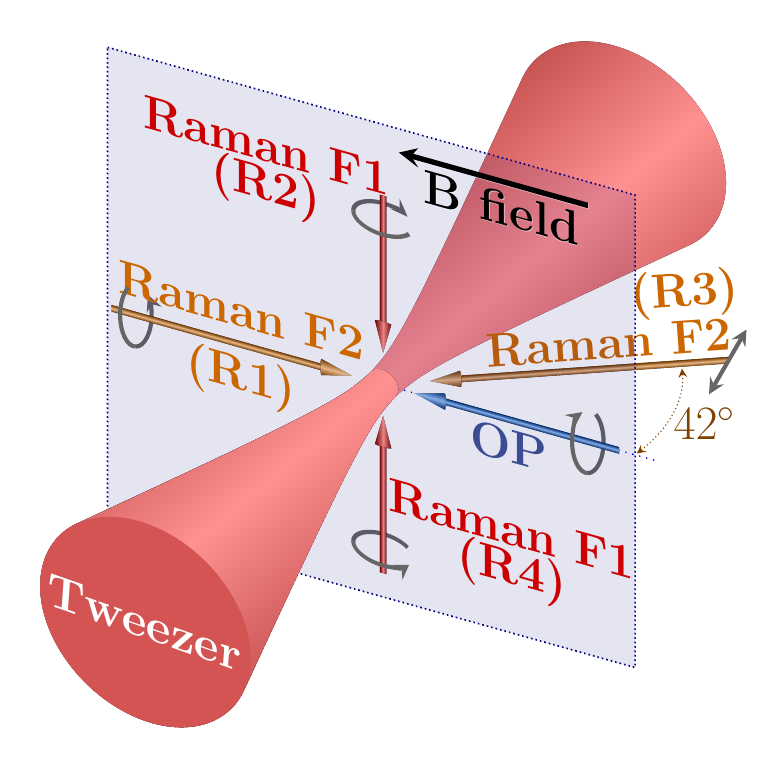
\begin{tikzpicture}
  \pgfmathsetmacro{\radiush}{1.5}
  \pgfmathsetmacro{\theight}{4}
  \pgfmathsetmacro{\radiusv}{.7 * \radiush}
  \pgfmathsetmacro{\waist}{.15}
  \pgfmathsetmacro{\xscale}{\radiush / sqrt(1 + (\waist)^2)}
  \pgfmathsetmacro{\radiusvs}{\radiusv / 0.9686}
  \pgfmathsetmacro{\radiushs}{\radiush / 0.9686}

  \fill[left color=red!50!black,right color=red!50!black,middle color=red!43,
  shading=axis,rotate=-45,shading angle=40]
  plot[domain={-1}:{1}, smooth, variable=\y]
  ({sqrt((\y)^2 + (\waist)^2) * \xscale}, \y * \theight)
  arc (-14.398:194.398:\radiushs cm and \radiusvs cm)
  -- plot[domain={-1}:{1}, smooth, variable=\y]
  ({-sqrt((\y)^2 + (\waist)^2) * \xscale}, -\y * \theight)
  arc (165.602:374.398:\radiushs cm and \radiusvs cm);

  \begin{scope}[transform canvas={rotate={4}}]
    \arrowthreeD{orange}{(0.6, 0)}{-90}{0.4}{3.4};
    \node[above,orange!80!black] at (2.9, 0) {\LARGE \textbf{Raman F2}};
    \node[above,orange!80!black] at (3.9, 0.45) {\LARGE \textbf{(R3)}};
  \end{scope}
  \draw[->,>=stealth,line width=1.5,color=black!60] (4:4.4) -- ++ (90-30:0.45);
  \draw[->,>=stealth,line width=1.5,color=black!60] (4:4.4) -- ++ (90-30:-0.5);

  \draw[orange!50!black, <->, densely dotted, >=stealth, line width=0.4]
  (3:3.8) arc (3:-32:3.8 and 1.85);
  \node[orange!50!black, right] at (-8:3.6) {\LARGE $42^\circ$};

  \draw[line width=1.5,color=black!60] (2.6, -0.40-2.6*0.28) arc (-90:60:0.20 and 0.40);
  \draw[->,>=stealth,line width=1.5,color=black!60]
  (-3.14, -0.40+3.14*0.28) arc (-90:40:0.20 and 0.40);

  \begin{scope}[transform canvas={cm={1,-0.28,0,1,(0, 0)}}]
    \draw[->,>=stealth,line width=1.5,color=black!60] (-0.38, 2.1) arc (180:35:0.38 and 0.20);
    \draw[line width=1.5,color=black!60] (-0.38, -2.1) arc (180:35:0.38 and 0.20);

    \draw[blue, dotted, line width=0.5] (0, 0) -- (3.5, 0);

    \fill[blue!50!black,opacity=0.1] (-3.5, 3.3) -- (3.2, 3.3)
    -- (3.2, -2.7) -- (-3.5, -2.7) -- cycle;
    \draw[blue!50!black, densely dotted,line width=0.6] (-3.5, 3.3) -- (3.2, 3.3)
    -- (3.2, -2.7) -- (-3.5, -2.7) -- cycle;
    \arrowthreeD{red}{(0, -0.4)}{180}{0.4}{1.6};
    \arrowthreeD{orange}{(-0.4, 0)}{90}{0.4}{2.65};
    \arrowthreeD{cyan!40!blue}{(0.4, 0)}{-90}{0.4}{2.2};
    \arrowthreeD{red}{(0, 0.4)}{0}{0.4}{1.6};
    \node[below,cyan!20!blue!80!black] at (1.6, 0) {\LARGE \textbf{OP}};
    \node[above,orange!80!black] at (-1.8, 0.1) {\LARGE \textbf{Raman F2}};
    \node[below,orange!80!black] at (-1.8, 0) {\LARGE \textbf{(R1)}};

    \node[left,red!80!black,align=center] at (0.2, 2.3)
    {\LARGE \textbf{Raman F1}\\\LARGE \textbf{(R2)}};
    \node[right,red!80!black,align=center] at (-0.05, -1.7)
    {\LARGE \textbf{Raman F1}\\\LARGE \textbf{(R4)}};

    \draw[white,opacity=0.5,->,>=stealth,line width=2] (2.61, 2.99) -- (0.21, 2.99);
    \draw[->,>=stealth,line width=2] (2.6, 3.0) -- (0.2, 3.0);
    \node[below,white,opacity=0.5] at (1.51, 2.99) {\LARGE \textbf{B field}};
    \node[below] at (1.5, 3.0) {\LARGE \textbf{B field}};

    \draw[line width=1.5,color=black!60] (-0.38, 2.1) arc (180:330:0.38 and 0.20);
    \draw[->,>=stealth,line width=1.5,color=black!60] (-0.38, -2.1) arc (180:330:0.38 and 0.20);
  \end{scope}

  \draw[->,>=stealth,line width=1.5,color=black!60]
  (2.6, -0.40-2.6*0.28) arc (-90:-250:0.20 and 0.40);
  \draw[line width=1.5,color=black!60]
  (-3.14, -0.40+3.14*0.28) arc (-90:-240:0.20 and 0.40);

  \begin{scope}
    \clip[rotate=-45]
    plot[domain={-1}:{0}, smooth, variable=\y] ({sqrt((\y)^2 + (\waist)^2) * \xscale}, \y * \theight)
    arc (0:180:{(\radiush)*(\waist)} and {(\radiusv)*(\waist)})
    -- plot[domain={0}:{1}, smooth, variable=\y] ({-sqrt((\y)^2 + (\waist)^2) * \xscale}, -\y * \theight)
    arc (165.602:374.398:\radiushs cm and \radiusvs cm);
    \fill[left color=red!50!black,right color=red!50!black,middle color=red!43,
    shading=axis,rotate=-45,shading angle=40]
    plot[domain={-1}:{1}, smooth, variable=\y]
    ({sqrt((\y)^2 + (\waist)^2) * \xscale}, \y * \theight)
    arc (-14.398:194.398:\radiushs cm and \radiusvs cm)
    -- plot[domain={-1}:{1}, smooth, variable=\y]
    ({-sqrt((\y)^2 + (\waist)^2) * \xscale}, -\y * \theight)
    arc (165.602:374.398:\radiushs cm and \radiusvs cm);
  \end{scope}

  \fill[red!60!gray!84!white,rotate=-45]
  ({-sqrt(1 + (\waist)^2) * \xscale}, -\theight)
  arc (165.602:{360+165.602}:\radiushs cm and \radiusvs cm) coordinate (Tweezer End);

  \begin{scope}[transform canvas={cm={1,-0.28,0,1,(0, 0)}}]
    \node[white,rotate=-4] at ($(Tweezer End) + (0.86, -2.1)$) {\LARGE \textbf{Tweezer}};
  \end{scope}
\end{tikzpicture}

\end{document}
